\documentclass[border=6pt]{standalone}
\usepackage{tikz}
\usepackage{amssymb}
\usepackage{lmodern}
\usetikzlibrary{positioning,arrows.meta,fit,backgrounds,calc}
\begin{document}
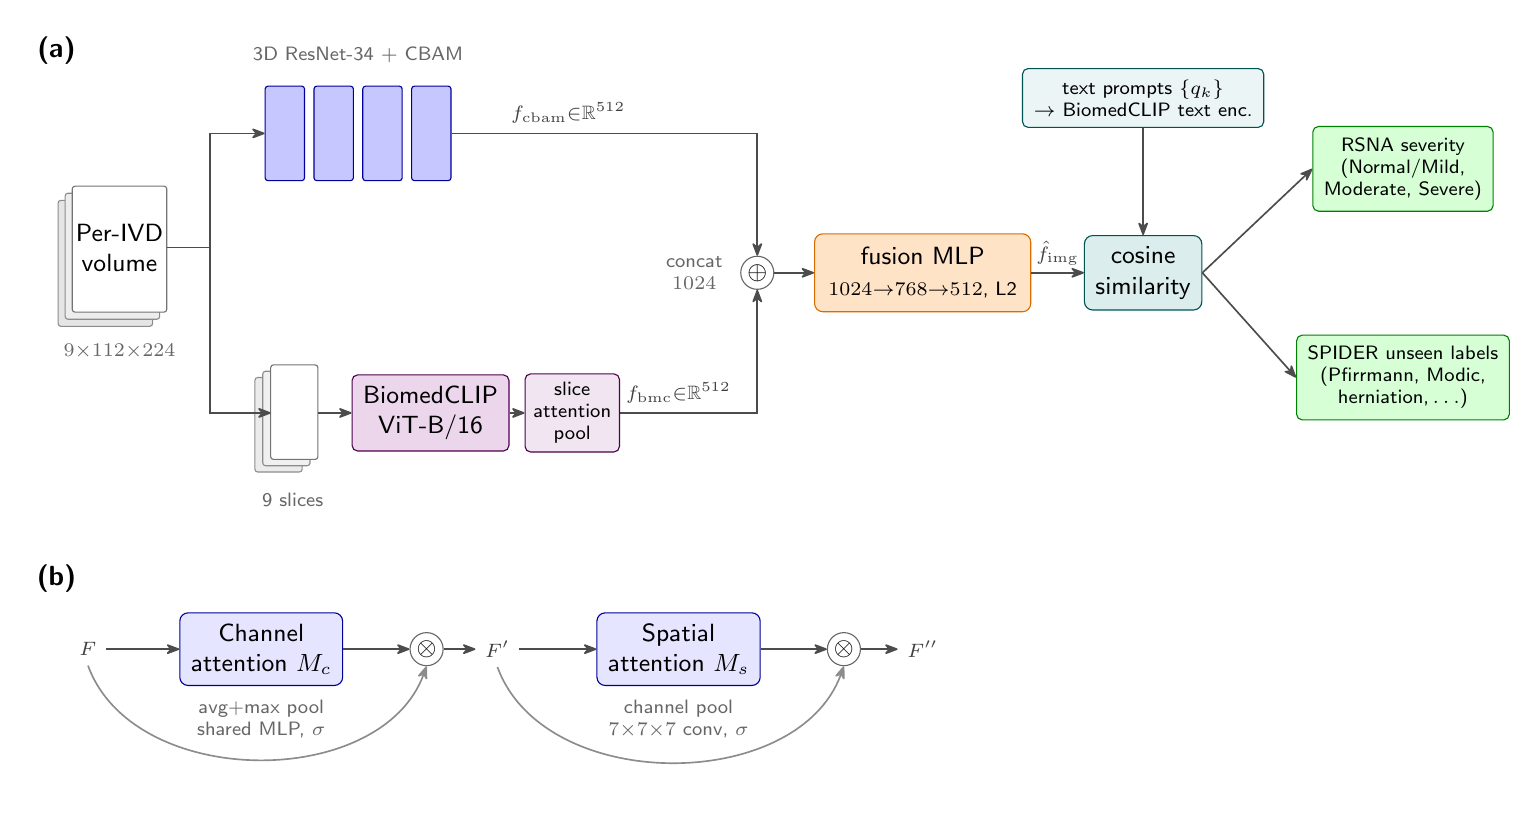
\begin{tikzpicture}[
  font=\sffamily,
  >={Stealth[round]},
  io/.style={rectangle,rounded corners=2pt,draw=black!55,fill=black!7,
             align=center,inner sep=4pt,font=\sffamily\small},
  cnn/.style={rectangle,rounded corners=1pt,draw=blue!60!black,fill=blue!22,
              minimum width=5mm,minimum height=12mm},
  vit/.style={rectangle,rounded corners=2pt,draw=violet!60!black,fill=violet!16,
              align=center,inner sep=4pt,font=\sffamily\small},
  proc/.style={rectangle,rounded corners=2pt,draw=violet!60!black,fill=violet!10,
               align=center,inner sep=3pt,font=\sffamily\scriptsize},
  fuse/.style={rectangle,rounded corners=3pt,draw=orange!85!black,fill=orange!22,
               align=center,inner sep=5pt,font=\sffamily\small},
  head/.style={rectangle,rounded corners=3pt,draw=teal!65!black,fill=teal!14,
               align=center,inner sep=4pt,font=\sffamily\small},
  outbox/.style={rectangle,rounded corners=2pt,draw=green!50!black,fill=green!16,
              align=center,inner sep=4pt,font=\sffamily\scriptsize},
  txt/.style={rectangle,rounded corners=2pt,draw=teal!65!black,fill=teal!8,
              align=center,inner sep=4pt,font=\sffamily\scriptsize},
  op/.style={circle,draw=black!60,inner sep=0pt,minimum size=4.2mm,font=\small},
  feat/.style={font=\sffamily\scriptsize,text=black!75},
  sub/.style={font=\sffamily\scriptsize,text=black!60,align=center},
  arr/.style={->,semithick,black!70}
]

% ===================== Panel (a): pipeline =====================
% ---- input volume (slice stack) ----
\begin{scope}
  \draw[draw=black!45,fill=black!10,rounded corners=1pt] (-0.18,-0.5) rectangle (1.02,1.1);
  \draw[draw=black!45,fill=black!7,rounded corners=1pt]  (-0.09,-0.41) rectangle (1.11,1.19);
  \draw[draw=black!55,fill=white,rounded corners=1pt]    (0,-0.32) rectangle (1.2,1.28);
\end{scope}
\node[align=center,font=\sffamily\small] (in) at (0.6,0.5) {Per-IVD\\volume};
\node[sub] at (0.6,-0.82) {$9{\times}112{\times}224$};

% ---- top branch: CBAM-3D ResNet-34 (mini stack) ----
\foreach \i in {0,1,2,3}{
  \node[cnn] (c\i) at (2.7+\i*0.62,1.95) {};
}
\node[sub] (cbamlab) at (3.63,2.95) {3D ResNet-34 $+$ CBAM};

% ---- bottom branch: BiomedCLIP ----
\begin{scope}
  \draw[draw=black!45,fill=black!8,rounded corners=1pt] (2.32,-2.35) rectangle (2.92,-1.15);
  \draw[draw=black!45,fill=black!6,rounded corners=1pt] (2.42,-2.27) rectangle (3.02,-1.07);
  \draw[draw=black!55,fill=white,rounded corners=1pt]   (2.52,-2.19) rectangle (3.12,-0.99);
\end{scope}
\node[sub] at (2.8,-2.7) {9 slices};
\node[vit] (vit) at (4.55,-1.6) {BiomedCLIP\\ViT-B/16};
\node[proc] (pool) at (6.35,-1.6) {slice\\attention\\pool};

% ---- fusion ----
\node[op] (cat) at (8.7,0.18) {$\oplus$};
\node[sub,left=1mm of cat] {concat\\\scriptsize$1024$};
\node[fuse] (mlp) at (10.8,0.18) {fusion MLP\\\scriptsize$1024{\to}768{\to}512$, L2};

% ---- cosine head + prompts + outputs ----
\node[head] (cos) at (13.6,0.18) {cosine\\similarity};
\node[txt] (prompt) at (13.6,2.4) {text prompts $\{q_k\}$\\$\to$ BiomedCLIP text enc.};
\node[outbox] (rsna) at (16.9,1.5) {RSNA severity\\\scriptsize(Normal/Mild,\\Moderate, Severe)};
\node[outbox] (spider) at (16.9,-1.15) {SPIDER unseen labels\\\scriptsize(Pfirrmann, Modic,\\herniation,\,$\dots$)};

% ---- arrows (panel a) ----
\draw[semithick,black!70] (1.2,0.5) -- (1.75,0.5);
\draw[arr] (1.75,0.5) |- (c0.west);
\draw[arr] (1.75,0.5) |- (2.52,-1.6);
\draw[arr] (3.12,-1.6) -- (vit.west);
\draw[arr] (vit.east) -- (pool.west);
\draw[arr] (c3.east) -- (8.7,1.95) -- (cat.north);
\draw[arr] (pool.east) -- (8.7,-1.6) -- (cat.south);
\node[feat,above] at (6.3,1.95) {$f_{\mathrm{cbam}}{\in}\mathbb{R}^{512}$};
\node[feat,above] at (7.7,-1.6) {$f_{\mathrm{bmc}}{\in}\mathbb{R}^{512}$};
\draw[arr] (cat.east) -- (mlp.west);
\draw[arr] (mlp.east) -- node[feat,above=-1pt]{$\hat f_{\mathrm{img}}$} (cos.west);
\draw[arr] (prompt.south) -- (cos.north);
\draw[arr] (cos.east) -- (rsna.west);
\draw[arr] (cos.east) -- (spider.west);

% ===================== Panel (b): CBAM block =====================
\def\by{-4.6}
\node[feat] (F) at (0.2,\by) {$F$};
\node[head,draw=blue!60!black,fill=blue!10] (mc) at (2.4,\by) {Channel\\attention $M_c$};
\node[sub,below=0.5mm of mc] {avg+max pool\\shared MLP, $\sigma$};
\node[op] (m1) at (4.5,\by) {$\otimes$};
\node[feat] (Fp) at (5.4,\by) {$F'$};
\node[head,draw=blue!60!black,fill=blue!10] (ms) at (7.7,\by) {Spatial\\attention $M_s$};
\node[sub,below=0.5mm of ms] {channel pool\\$7{\times}7{\times}7$ conv, $\sigma$};
\node[op] (m2) at (9.8,\by) {$\otimes$};
\node[feat] (Fpp) at (10.8,\by) {$F''$};

\draw[arr] (F) -- (mc);
\draw[arr] (mc) -- (m1);
\draw[arr] (m1) -- (Fp);
\draw[arr] (Fp) -- (ms);
\draw[arr] (ms) -- (m2);
\draw[arr] (m2) -- (Fpp);
% residual feature lines into the multiply ops
\draw[arr,black!45] (F.south) to[out=-70,in=-110] (m1.south);
\draw[arr,black!45] (Fp.south) to[out=-70,in=-110] (m2.south);

% ---- panel captions ----
\node[font=\sffamily\bfseries] at (-0.2,3.0) {(a)};
\node[font=\sffamily\bfseries] at (-0.2,-3.7) {(b)};

\end{tikzpicture}
\end{document}
